% !TeX encoding = UTF-8

\chapter{FUNDAMENTAÇÃO TEÓRICA}\label{ch:fundaments-teorico}
Nos tópicos que seguem, serão apresentados conceitos teóricos sobre o tema proposto. Ou seja, será realizada uma fundamentação desde o processo de funcionamento de RNAs até sua aplicabilidade no mercado acionário.

%%
% FUNDAMENTOS
\section{FUNDAMENTOS DE REDES NEURAIS ARTIFICIAIS}\label{sec:fundamentos}
As RNAs procuram simular métodos de aprendizado do cérebro humano, através do uso de neurônios interligados. Uma RNA é inspirada nos neurônios biológicos e nos sistemas nervosos, logo, para entender o funcionamento da mesma, é necessário, primeiramente, entender o funcionamento dos neurônios biológicos \cite{neto}.

A partir deste conceito, uma RNA pode ser definida como uma estrutura interligada complexa de processamento, composta por neurônios e conexões \cite{ferreira}.

\subsection{Neurônios biológicos} 
Os neurônios são células, que desempenham o papel de conduzir os impulsos nervosos. Estas células especializadas são, portanto, as unidades básicas do sistema que processa as informações e estímulos de um cérebro\cite{lent}. 

A Figura 1 representa a estrutura básica de um neurônio biológico. Conceituando os componentes do neurônio, os dendritos são responsáveis pela recepção das informações, possuindo as extremidades ramificadas. O corpo celular é responsável pela integração das informações e os axônios são responsáveis pelo transporte dos impulsos nervosos de um neurônio para outro ou de um neurônio para uma glândula ou fibra muscular \cite{lent}.

\begin{figure}[h]
	\centering
	\fbox{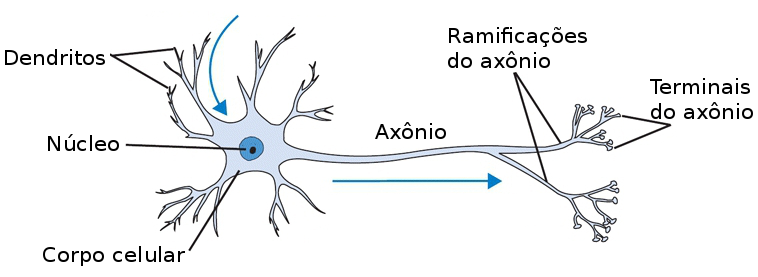
\includegraphics[width=0.6\textwidth]{cerebro}}
	\caption{Representação de um neurônio biológico}
	\fonte{Adaptado de \citeonline{stanford} }
	\label{exec-linearmente-separavel}
\end{figure} 

Cada dendrito possui em torno de mil a dez mil ramificações em suas extremidades. A transmissão de impulsos nervosos por meio da comunicação dos axônios com os dendritos de neurônios adjacentes é chamada de sinapse, por sua vez, tal conjunto forma o sistema nervoso \cite{neto}.

\subsection{Neurônios artificiais}
A estrutura de um neurônio artificial segue os mesmos conceitos relacionados aos neurônios biológicos, buscando realizar as mesmas funções, utilizando-se de conceitos matemáticos, aritméticos e de tecnologias computacionais.

A Figura 2 esboça a estrutura que compõe um neurônio artificial não-linear, demarcando cada item que o compõe. 

\begin{figure}[h]
	\centering
	\fbox{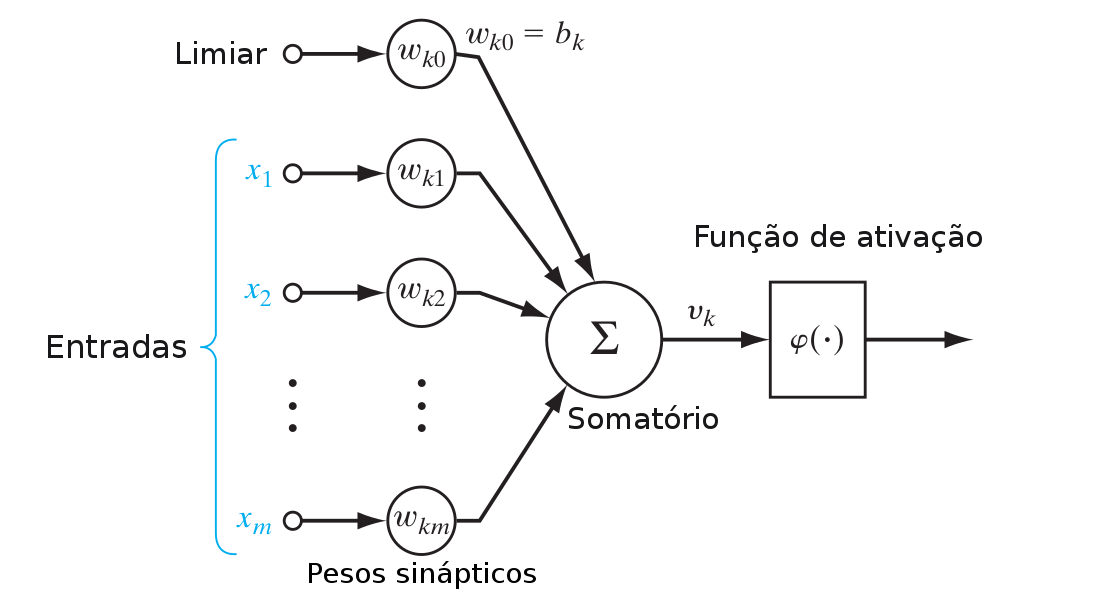
\includegraphics[width=0.8\textwidth]{neuronio}}
	\caption{Representação de um neurônio artificial}
	\fonte{Adaptado de \citeonline{haykin2009} }
	\label{exec-linearmente-separavel}
\end{figure}

Analisando a figura da esquerda para a direita, podemos observar: 

\begin{enumerate}
	\item \textit Os sinais de entrada $x_i$ serão processados pela sinapse $wk_i$, conectadas ao neurônio;
	\item \textit As sinapses ou elos de conexão, com seus respectivos pesos sinápticos que se multiplicarão ao sinal de entrada $\theta_i$. Segundo \citeonline{haykin2000}, ao contrário a uma sinapse do cérebro, o peso sináptico de um neurônio artificial pode estar em um intervalo que inclui tanto valores positivos quanto negativos;
	\item \textit O somatório $\sum$, que resulta na soma dos sinais de entrada $x_i$, ponderados pelas respectivas sinapses do neurônio;
	\item \textit A função de ativação, responsável por delimitar os resultados de saída possíveis a um intervalo finito, recebe como entrada o resultado $v_k$ em $\varphi$(.) para gerar o resultado.
\end{enumerate}

\subsection{Redes Neurais Artificiais}\label{sec:redes-neurais}
Uma RNA pode ser definida como uma ferramenta computacional, produzida e programada para realizar análise de dados, tal como seu comportamento e relações, visando trabalhar com os mesmos conceitos de um sistema nervoso, simulando o comportamento de um conjunto de neurônios biológicos. Por meio de complexos processos de treinamento e aprendizagem, as RNAs visam realizar o reconhecimento de padrões de dados, para que possa prever resultados, através de classificação ou generalização dos dados em questão \cite{haykin2009}.

A representação de uma RNA pode ser visualizada na Figura 3, onde os nodos do grafo representam os neurônios, as arestas representam as conexões e as setas representam a direção do fluxo de sinal.

\begin{figure}[h]
	\centering
	\fbox{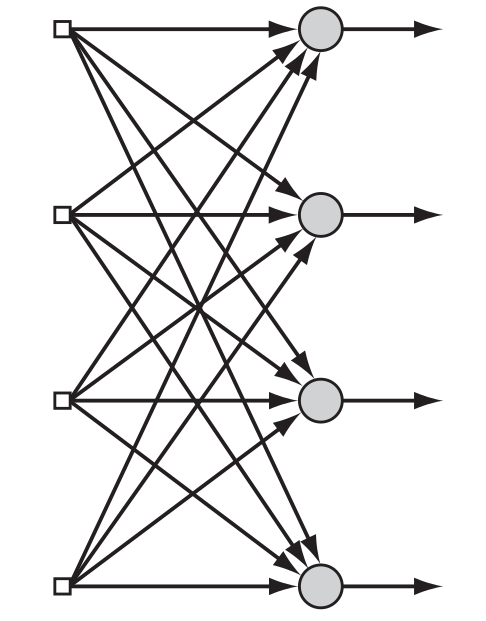
\includegraphics[width=0.5\textwidth, height=0.33\textheight]{RNA}}
	\caption{Representação gráfica de uma Rede Neural Artificial}
	\fonte{\citeonline{haykin2009}}
	\label{exec-rna}
\end{figure}

\section{ARQUITETURA DE REDES NEURAIS ARTIFICIAIS}\label{sec:redes-neurais-arquitetura}
A forma como agrupam-se os neurônios artificiais em uma RNA é uma das principais características que definem seu tipo de arquitetura. Estes agrupamentos são baseados na forma como os neurônios são conectados no cérebro humano, de forma que as informações possam ser processadas dinamicamente ou iterativamente.
 
Biologicamente, as RNAs são organizadas e construídas de forma tridimensional por componentes microscópicos. Há uma forte restrição no número de camadas que a rede pode conter, limitando consideravelmente o tipo e o escopo da implementação da mesma, dependendo da complexidade do problema \cite{haykin2009}.

A arquitetura de uma RNA pode ser classificada pela quantia de camadas ocultas e pelo sentido do fluxo de dados. Em relação ao número de camadas ocultas, ela pode ser de camada única (\textit{single-layer}) ou multicamadas (\textit{multilayer}). Quanto ao sentido do fluxo de dados, ela pode ser alimentada adiante (\textit{feedforward}) ou recorrente (\textit{feedback}) \cite{neto}.

As redes que possuem uma única camada são as que possuem um nó entre sua entrada e saída. Este tipo de rede é indicada para a solução de problemas linearmente separáveis. Já as que possuem multicamadas apresentam uma ou mais camadas entre seu início e fim. Essas camadas são chamadas de camadas escondidas (\textit{hidden}, intermediárias ou ocultas).

A topologia de RNA mais popular atualmente é a rede direta com neurônios estáticos (\textit{feedforward}) juntamente com a perceptron de múltiplas camadas (\textit {Multilayer Perceptron}) que utiliza o algoritmo de retropropagação (\textit{backpropagation}) como forma de treinamento \cite{neto}.

\subsection{Redes Alimentadas Adiante com Camada Única}
A organização de uma RNA em camadas adiante pode ser representada de uma maneira simples, onde os neurônios, distribuídos em camadas, recebem sinais de entrada que são projetados sobre os mesmos. Porém, nesta distribuição não ocorre o contrário, ou seja, o fluxo de alimentação ocorre sempre no sentido adiante ou acíclico.
 
Segundo \citeonline{haykin2000}, na estrutura de camada única, a representação dos nós de neurônios responsáveis por receber e processar os sinais de entrada é dada em uma única camada. Para melhor entendimento deste tipo de estrutura, a Figura 4 exemplifica um modelo de RNA com essa característica.

\begin{figure}[h]
	\centering
	\fbox{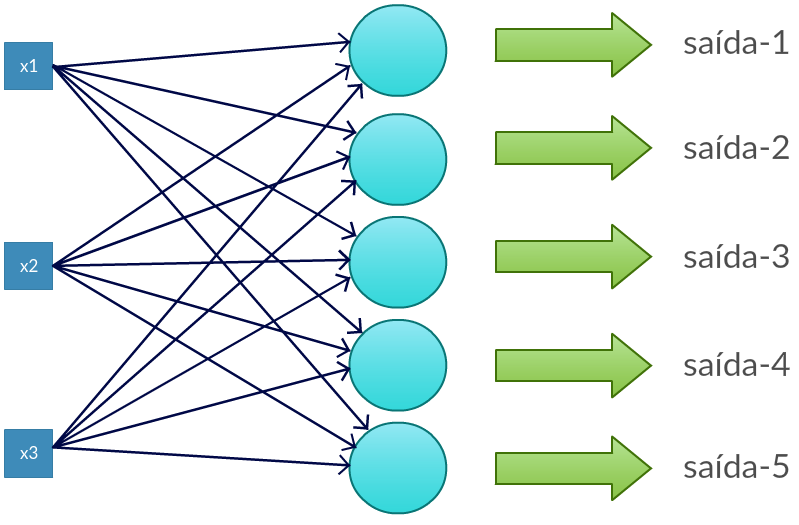
\includegraphics[width=0.6\textwidth]{camadaunica}}
	\caption{Representação de uma Rede Neural Artificial com camada única}
	\fonte{Elaborado pelo autor}
	\label{exec-rna-camada-unica}
\end{figure}

Para exemplificar este modelo de camada única, pode-se citar a RNA \textit{Perceptron} simples, criada por Frank Rosenblatt em 1957 nos laboratórios das forças militares. A classificação dos resultados de uma RNA desta categoria é ilustrada na Figura 5, onde seus resultados são linearmente separáveis. Ou seja, este modelo de RNA é capaz de classificar de forma satisfatória, resultados que podem ser separados por uma reta ou hiperplano como fronteira de decisão \cite{haykin2009}.

\begin{figure}[h]
	\centering
	\fbox{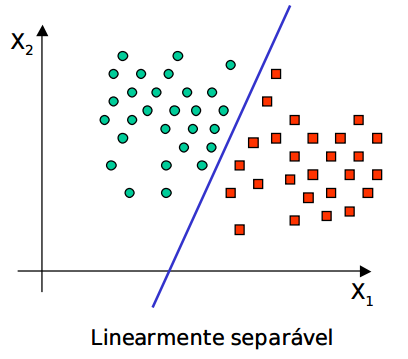
\includegraphics[width=0.5\textwidth]{separavel}}
	\caption{Representação de resultados linearmente separáveis}
	\fonte{\citeonline{oliveira2002} }
	\label{exec-linearmente-separavel}
\end{figure}

\subsection{Redes Alimentadas Adiante com Múltiplas Camadas}
A estrutura de múltiplas camadas, difere-se da primeira classe alimentada adiante em relação a composição de suas camadas. Esta classe de redes surgiu da necessidade em aperfeiçoar a capacidade de mapeamento que um modelo de camada única não proporciona. Um exemplo clássico é a função ou-exclusivo (XOR) \cite{haykin2009}.

Tipicamente, a rede consiste em uma camada de entrada, uma ou mais camadas ocultas e uma camada de saída. O sinal de entrada se propaga para frente através da rede, camada por camada. Este tipo de rede é bastante popular devido aos métodos de aprendizado bem distribuídos e de fácil uso \cite{haykin2000}.

Sua representação pode ser vista na Figura 6, onde pode-se observar a presença de duas camadas intermediárias até a apresentação de seu resultado.

De acordo com \citeonline{haykin2000}, qualquer rede semelhante à representada na Figura 6, é dita totalmente conectada, visto que todas as entradas $x_i$ se conectam a todos os nós da camada oculta $a_i$. Caso a premissa não fosse estabelecida a rede seria dita parcialmente conectada.

Outro ponto que a difere da classe com camada única, é a possibilidade de trabalhar com problemas não-lineares. Ou seja, os resultados não necessariamente são classificados de forma satisfatória através apenas de uma reta ou hiperplano, o que aumenta a capacidade de RNAs com esta característica em resolver problemas mais complexos.

\begin{figure}[h]
	\centering
	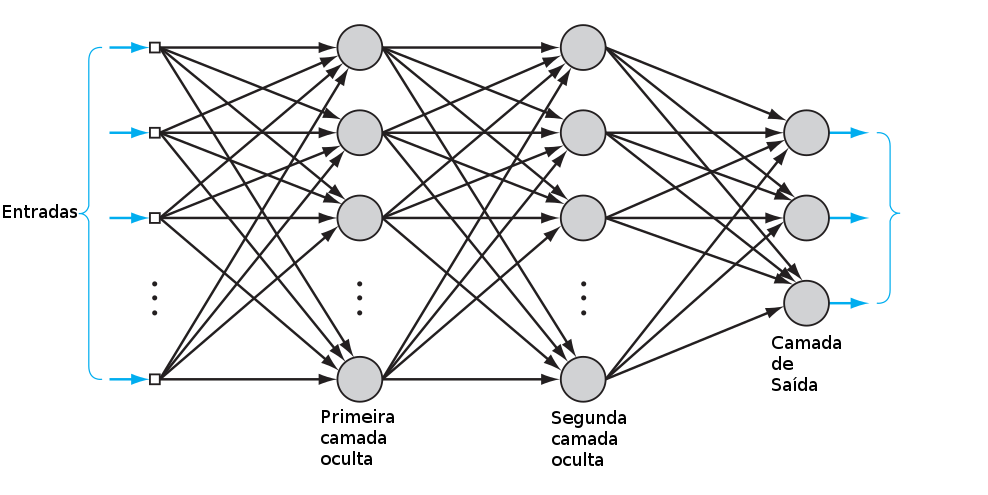
\includegraphics[width=0.9\textwidth]{multicamada}
	\caption{Rede Neural Artificial com múltiplas camadas}
	\fonte{Adaptado de \citeonline{haykin2009}}
	\label{fig-multiplas-camadas}
\end{figure}

A Figura 7 exemplifica a representação de um resultado não-linear proporcionado por uma rede de múltiplas camadas.

\begin{figure}[h]
	\centering
	\fbox{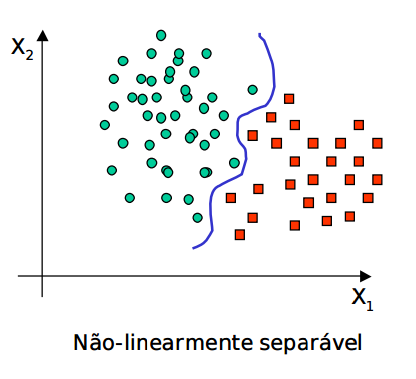
\includegraphics[width=0.5\textwidth]{naolinear}}
	\caption{Classificação de resultados não-lineares}
	\fonte{\citeonline{oliveira2002}}
	\label{exec-nao-linear-imagem}
\end{figure}

\subsection{Redes de Camadas Recorrentes}
Diferentemente da arquitetura de camadas simples adiante, a arquitetura de camadas recorrentes apresenta ao menos um laço de realimentação. A presença de realimentação de informação permite a criação de representações internas e dispositivos de memória capazes de processar e armazenar informações temporais e sinais seqüenciais. Em seu trabalho, \citeonline{haykin2000} cita um exemplo clássico de uma rede de camadas recorrentes, onde os neurônios em camada única alimentam seus sinais de saída novamente para as entradas de todos os neurônios.

A arquitetura de uma RNA recorrente pode ser observada na Figura 8, onde as entradas são realimentadas através da saída. Após realizado esse processamento, a rede apresenta o resultado calculado.

\begin{figure}[h]
	\centering
	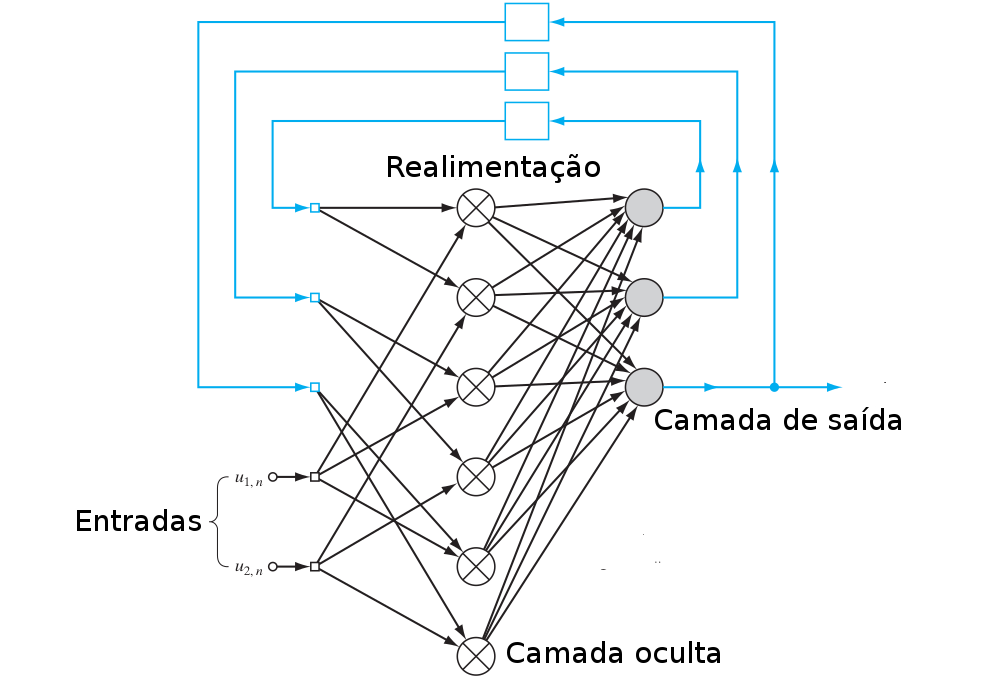
\includegraphics[width=.9\textwidth]{recorrente}
	\caption{Rede Neural Artificial recorrente}
	\fonte{Adaptado de \citeonline{haykin2009} }
	\label{fig-recorrente}
\end{figure}

\subsection{Redes de Hopfield}
Dentre outros modelos e arquiteturas de redes que existem, pode-se citar Hopfield, desenvolvida pelo físico John Hopfield. Este modelo se caracteriza por ser do tipo \textit{feedback}, por este motivo, estas redes dificilmente chegam a um estado instável, pois chegará um momento, após seu treinamento, em que o valor de saída para determinadas entradas se padronizam, alcançando sua estabilidade. O modelo utilizou uma função de energia como ferramenta para desenhar redes recorrentes e entender como funciona seu comportamento dinâmico. Desta forma, popularizou o uso desta arquitetura como uma memória associativa e para resolver problemas de otimização \cite{cardon}.

O modelo aplica um princípio chamado de armazenamento de informação como atratores dinamicamente estáveis. Para recuperar informações, utilizou um processo dinâmico de atualização dos estados dos neurônios, sendo que, o neurônio a ser atualizado, é escolhido aleatoriamente. Dois modelos de redes foram apresentados por Hopfield: o analógico e o binário \cite{silva}.

\subsection{Redes Auto-Organizáveis}
Segundo \citeonline{haykin2009}, Redes Auto-Organizáveis são modelos de 2 camadas que aceitam padrões de N-dimensões como entrada e os mapeia para um conjunto de neurônios de saída, o qual representa o espaço dos dados a serem agrupados. O mapa (camada) de saída, que é tipicamente bi-dimensional, representa as posições dos neurônios em relação aos seus vizinhos. A ideia é que neurônios topologicamente próximos respondam de maneira semelhante a entradas semelhantes. Para isso todos neurônios da camada de entrada são todos conectados aos neurônios de saída.

\section{FUNÇÃO DE ATIVAÇÃO}\label{sec:funcao-ativacao}
O processamento em cada neurônio se dá através da função de ativação. A escolha da função de ativação de uma RNA é um processo de grande relevância, uma vez que esta função define como devem ser tratados seus dados de entrada. As funções de ativação podem ser classificadas como lineares ou não lineares \cite{haykin2000}.

Segundo \citeonline{haykin2000}, caracterizando-se pela limitação de valores de saída a um intervalo finito, destacam-se os modelos de funções: limiar, sigmóide e tangente hiperbólica.

\subsection{Função Limiar}
Para este exemplo de função temos que para:
 
\begin{equation}\label{eq:limiar}
y=\sum_{j=1}^{w} w_{kj}\ x_j + b_{k'}
\end{equation}

Onde $x$ é a entrada induzida no neurônio, gerando um resultado $y_k$ dado por:
\begin{equation}\label{eq:limiar-result} 
y_k = {1\ se\ x_j  > 0}
\end{equation}

ou
\begin{equation}\label{eq:limiar-result} 
y_k = {0\ se\ x_j < 0}  
\end{equation}

Neste modelo a saída do neurônio assume o valor 1 se o campo local induzido daquele neurônio for positivo, e 0 se for negativo. Utilizam-se dos mesmos preceitos de regressão linear e de outras técnicas, para estimar resultados a partir de valores conhecidos.

\subsection{Função Sigmóide}
A função sigmóide, representada na Equação (3.4), é a forma mais comum de função de ativação utilizada na construção de RNAs.
\begin{equation}\label{eq:limiar-result} 
f(x)=\frac{1}{1+e^{- \lambda x}}
\end{equation}

Onde $- \lambda x$ é a entrada a ser processada.

\citeonline{haykin2009} define a função sigmóide como uma função crescente, com o  objetivo de realizar um balanceamento adequado entre comportamentos lineares e não-lineares em um intervalo entre [0,1] justificando sua grande usabilidade. No Código 1 é apresentada a implementação da função na linguagem de programação Python.

\citeonline{haykin2009} também evidência a utilização da tangente hiperbólica com o mesmo intuito da sigmóide, porém com um intervalo variando em um intervalo de [-1,1].

\codigoPython\
\lstinputlisting[label=cod:exempla-sigmoide, caption=Função sigmóide em Python]{src/Sigmoide.py}

Resultados com esta característica são reconhecidos por formar um "S", exemplificado no Gráfico 1.

\begin{grafico}[h]
	\centering
	\fbox{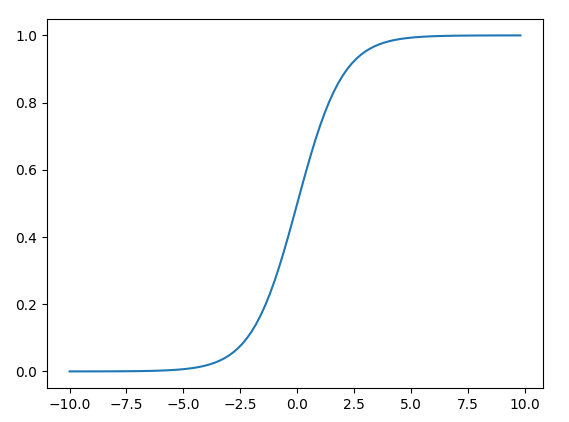
\includegraphics[width=0.8\textwidth]{sigmoide}}
	\caption{Comportamento de uma função sigmóide}
	\fonte{Elaborado pelo autor}
	\label{sigmoide-graph}
\end{grafico}


\section{TREINAMENTO DE UMA REDE NEURAL ARTIFICIAL}\label{sec:rna-treinamento}
Após determinar a arquitetura a ser utilizada pela RNA, a quantia de camadas, a função de ativação adequada ao trabalho a ser realizado, a rede neural deve adquirir conhecimento em relação aos dados aplicados sobre a mesma.

O treinamento de uma RNA consiste em minimizar uma função de custo, através de um algoritmo, cujos valores iniciais são escolhidos aleatoriamente com o objetivo de facilitar a busca  pelo valor mínimo da função da amostra de treinamento, através de iterações, este processo é conhecido como mínimo global. O treinamento pode ser interrompido de duas formas: Um limite de épocas estipulado para o treinamento ou um ponto de parada a partir de um critério de desempenho. Os critérios de desempenho típicos em um processo de treinamento de uma determinada amostra de dados, são o Erro quadrático médio (EQM), Raiz do Erro Quadrático Médio (REQM) e o Erro Absoluto Médio (EAM) \cite{gambogi}. 

\subsection{Processo de aprendizagem}
O processo de aprendizagem é considerado uma etapa de grande dificuldade em termos de análise de dados, porque a procura da solução adequada ocorre em um universo de soluções válidas de grande dimensão, onde a base de tomada de decisão serão os próprios dados treinados \cite{medeiros}.
 
Para adquirir conhecimento, uma RNA requer um processo de inúmeras iterações e aprendizagem, absorvendo os conhecimentos sobre o comportamento e relacionamento dos dados a cada iteração e armazenando os ajustes realizados nos pesos sinápticos de cada neurônio \cite{neto}.

Segundo \citeonline{haykin2000}, o processo de aprendizagem de uma rede neural pode ser resumido a uma sequência de três passos a cada estímulo enviado a rede, são eles:

\begin{enumerate}
	\item \textit O ambiente estimula a RNA com informações oriundas do mundo exterior;
	\item \textit A RNA experimenta alterações em seus pesos na tentativa de melhor responder ao estímulo recebido;
	\item \textit A RNA responde ao estímulo recebido após empreender as alterações realizadas no evento anterior.
\end{enumerate}

A cada estímulo enviado a RNA em sua aprendizagem, a sequência acima é realizada, os pesos sinápticos são ajustados até que atinjam seus valores ideais, visando aumentar a acuracidade dos resultados do processo, este processo, segundo \citeonline{haykin2000}, é conhecido como algoritmo de aprendizagem.

\subsubsection{Aprendizagem Supervisionada}
Nesse modelo de aprendizagem, o acompanhamento dos resultados é supervisionado constantemente durante o processo de treinamento e aprendizagem da rede. Nele, é disponibilizado o resultado esperado em relação aos dados aplicados na RNA. Logo, estima-se a qualidade dos resultados obtidos de acordo com o desvio do padrão de resultados obtidos em relação aos aguardados \cite{haykin2009}.

\subsubsection{Aprendizagem não Supervisionada}
No modelo de aprendizagem não supervisionada, não há supervisão dos dados processados, tal como não é disponibilizado um modelo de resultados esperados na aplicação em questão.

Segundo \citeonline{haykin2009}, dentre as existentes destacam-se duas formas de aprendizagem não supervisionadas, são elas: aprendizagem por reforço e aprendizagem auto-organizada. A primeira delas está diretamente relacionada à métodos de programação dinâmica. Já a segunda, está relacionada a aprendizagem competitiva, método onde os neurônios são postos de forma que compitam entre si, sendo somente um deles ativado no ciclo de aprendizagem.

\section{ALGORITMOS DE APRENDIZAGEM PARA TREINAMENTO DAS REDES}\label{algoritmos-aprendizagem}
Muitos algoritmos são aplicados para a minimização e melhoria da aprendizagem da RNA. Esses algoritmos podem ser classificados como de minimização local e minimização global. Algoritmos de minimização local, tal qual o método gradiente descendente, são rápidos, porém convergem para mínimos locais. Por outro lado, os algoritmos de minimização global usam estratégias heurísticas para escapar dos mínimos locais \cite{haykin2000}.

\subsection{\textit{Backpropagation}}
O algoritmo de retropropagação (\textit{backpropagation}) é um método baseado no gradiente descendente, de aprendizado supervisionado e com alimentação à frente, que utiliza a função de ativação do tipo sigmóide e um coeficiente de aprendizado, denominado \textit{learning rate}, responsável por especificar uma taxa de convergência da RNA, este coeficiente de aprendizado normalmente está em um intervalo entre [0,1]    \cite{haykin2000}.
Neste modelo, reconhecido por ser a técnica mais utilizada dentre os métodos de treinamento aplicados, o erro de saída obtido se propaga para as camadas intermediárias da RNA, isso se dá pela necessidade de ajuste dos neurônios que não tem contato com a saída, possibilitando assim, a atualização dos pesos desses neurônios, aumentando o poder de classificação e de correção de erros \cite{medeiros}.

O algoritmo usa a Equação abaixo para atualizar os pesos de um determinado neurônio.
\begin{equation}\label{eq:backpropagation-ajuste-pesos}
W_{ij,(t+1)} = W_{ij, t} + (\lambda)(\varepsilon W_{ij})(N_i)
\end{equation}

A equação 3.5 realiza a atualização do peso $W_{ij}$ de um determinado neurônio $N_i$ referente ao neurônio atual $N_j$ , onde o sub-índice $t$ refere-se ao número de vezes em que a rede foi atualizada e $\lambda$ refere-se à taxa de aprendizagem (\textit{learning rate}). Esta taxa de aprendizagem é responsável por controlar o peso e suas alterações.	

\section{PROCESSO DE GENERALIZAÇÃO}\label{rna-generalização}
O processo de generalização de uma RNA, ocorre a partir da sua capacidade em responder adequadamente não somente aos padrões de treinamento mas também aos demais padrões \cite{medeiros}. Vale ressaltar que o processo de treinamento é uma das etapas mais delicadas, em termos de análise e execução, ao se utilizar um modelo de RNA.

Tendo este conceito como ponto de partida, a capacidade de alta generalização desses modelos são fatores fundamentais para alcançar um nível de excelência. Ou seja, desde os primórdios destas técnicas, são utilizados métodos que possam abstrair a complexidade e suprir a necessidade de controlar o processo de generalização.

\subsection{Problemas de generalização}
 Diferentes realizações para um conjunto de treinamento podem fazer com que diferentes soluções sejam tomadas, dada uma topologia de rede. Essa variabilidade de soluções, dados os conjuntos de treinamentos distintos para uma mesma tarefa, é chamada de variância \cite{haykin2000}.
 
Para garantir uma boa capacidade de generalização, a idéia é minimizar ao máximo essa variância que ocorre no processo de treinamento \cite{medeiros}. As inconsistências que influenciam  na capacidade de generalização de um algoritmo podem ser atribuídas aos seguintes fatores: sobre-ajuste (\textit{overfitting}), sub-ajuste (\textit{underfitting}) e sobretreinamento (\textit{overtraining}). A seguir encontram-se alguns detalhes a respeito desses fatores.

\subsubsection{\textit{Overfitting} e \textit{underfitting}}
As soluções que apresentam inconsistências devido à alta taxa de variância geralmente apresentam sobre-ajuste em relação aos dados de treinamento, efeito conhecido como overfitting \cite{medeiros}. Na Figura 9 pode-se observar o comportamento de uma função com \textit{overfitting}.

Uma forma de evitar a alta taxa de variância, e assim, a ocorrência de \textit{overfitting}, se dá pela simplificação dos parâmetros de ativação da RNA. Porém, a redução desses parâmetros podem ocasionar outro problema muito comum dentre os protótipos desenvolvidos, denominado \textit{underfitting}. \textit{Underfitting} refere-se a um modelo que não pode nem modelar os dados de treinamento nem generalizar a novos dados, tornando-se um modelo estático, limitando assim, sua característica de aprender novos padrões \cite{geman}. Na Figura 9 pode-se observar o comportamento de uma função com \textit{underfitting}.

Com isso nota-se que deve existir um ponto de equilíbrio entre ambos efeitos, várias são as abordagens que tentam minimizar esses problemas, como os métodos construtivos e os algoritmos de \textit{pruning}.

Os algoritmos construtivos buscam a construção gradual da RNA por meio da adição, até que um critério de parada envolvendo o erro de treinamento seja atingido. A resposta da rede se inicia em uma situação de \textit{underfitting} e com a adição de novos neurônios aproxima-se de \textit{overfitting}, a idéia desses algoritmos consiste em encontrar uma melhor generalização na transição entre esses dois extremos \cite{medeiros}.

Os algoritmos de pruning, por sua vez, visam à minimização da estrutura pela eliminação gradativa dos pesos e dos neurônios, buscando diminuir os pesos excessivos, e assim, diminuindo o \textit{overfitting}.

\begin{figure}[h]
	\centering
	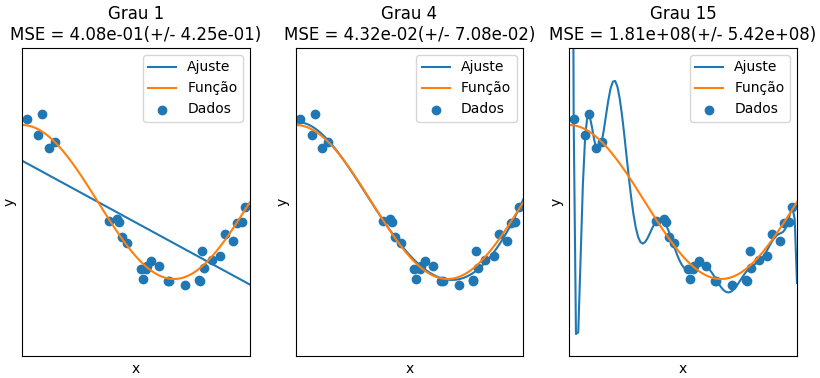
\includegraphics[width=0.9\textwidth]{overfitting}
	\caption{Comportamento de funções com \textit{overfitting} e \textit{underfitting}}
	\fonte{Elaborado pelo autor}
	\label{overfittin-fig}
\end{figure}

\subsubsection{\textit{Overtraining}}
As arquiteturas convencionais de treinamento estão sujeitas a sofrerem um sobretreinamento (\textit{overtraining}). Quando a rede parece estar respondendo o conjunto de dados cada vez melhor, ou seja, o erro de treinamento do conjunto de dados continua diminuindo, em algum ponto desse processo, a capacidade em resolver novos padrões torna-se falha. Isto ocorre por utilizar dados muito parecidos, assim como a quantidade de épocas em que esse conjunto de dados é treinado, viciando o conhecimento da RNA \cite{haykin2000}.

\section{TEORIA DA REGULARIZAÇÃO}\label{regularizacao}
A regularização é um método que busca melhorar a capacidade de generalização dos algoritmos de aprendizado por meio de alguma regra durante o processo de treinamento. A idéia básica da regularização é estabilizar a solução por meio de uma suavização entre o mapeamento da entrada até a saída, no sentido de que entradas similares correspondam a saídas similares. A suavização pode transformar um problema mal posto em um problema bem posto \cite{medeiros}. Um dos problemas a ser resolvido com métodos de regularização, seria encontrar um ponto de equilíbrio entre \textit{overfitting} e \textit{underfitting} no processo de treinamento de uma RNA, implicando na suavização do conjunto de dados.

\section{SÉRIES TEMPORAIS}\label{series-temporais}
Séries temporais são definidas como sequências de dados indexados ao longo de um período. Diferentemente de dados em seção transversal (\textit{cross-section}), em que os dados são coletados somente em um determinado instante de tempo, representando uma instância dos dados naquele momento, a ordem temporal dos dados tem relevância na obtenção de resultados e conclusões. Se a ordem dos dados for modificada, haverá perda de informação relevante sobre os dados, podendo obter conclusões equivocadas em relação à série em estudo \cite{neto}.

As séries temporais podem ser classificadas de diversas formas. Elas podem ser contínuas, quando a sequência de dados é descrita continuamente no tempo, e discretas, quando a sequência de dados é descrita em instantes de tempo discretos, havendo um espaçamento entre os instantes. A classificação em discreta e contínua é em relação ao tempo e não ao valor de cada observação. Pode-se ter uma série temporal discreta, mas o conteúdo das suas variáveis ser contínuo. Na prática, a utilização de séries temporais econômicas e financeiras é dada na forma discreta, pois, a coleta de dados é viabilizada em instantes de tempo discretos \cite{oliveira2012}.

\section{MERCADO DE CAPITAIS}\label{capitais}
O mercado de capitais é um sistema de distribuição de valores mobiliários que visa proporcionar liquidez aos títulos de emissão de empresas e viabilizar seu processo de capitalização. É constituído pelas bolsas, corretoras e outras instituições financeiras autorizadas \cite{tororadar}.

Os mercados de grandes ações são considerados os pilares centrais do crescimento e desenvolvimento econômico. Prever como irá se comportar futuramente o movimento de ações, tornou-se interesse comum entre investidores deste mercado \cite{pereira}.

Partindo deste pretexto, estudos ligados a predição de valores do mercado acionário, dividem-se basicamente em três vertentes. Há os que não crêem que investidores podem conseguir consideráveis vantagens em transações, que se fundamentam em teorias aleatórias de mercado. Há também os que crêem no hábito de seguir aspectos relacionados a análise fundamentalista de empresas e indicadores macro-econômicos. Por fim, há os que crêem que com base em séries recentes de dados e históricos é possível conseguir generalizar e classificar padrões de dados. A partir da última citação, surgem os interesses em trabalhos que relacionam o tema à técnicas de inteligência computacional, especificamente o uso de redes neurais artificiais \cite{pereira}.

\subsection{Análise Fundamentalista de Acões}
Antes da realização de qualquer investimento no mercado acionário é fundamental que sejam analisados itens de considerável importância no ramo financeiro, como indicadores de balanço e de mercado. O objetivo da análise é de reconhecer previamente as altas e baixas de determinadas ações em um período de tempo.

A análise fundamentalista busca, basicamente, avaliar a saúde financeira das empresas, projetar seus resultados futuros e determinar o preço justo para as suas ações. Para isso, os analistas levam em consideração os chamados fundamentos da empresa, isto é, todos os fatores macro e microeconômicos que influenciam no seu desempenho. A partir de uma minuciosa análise de todos eles, é possível projetar os resultados da companhia a longo prazo, em geral num período de cinco a dez anos \cite{exame}.

\subsection{Análise Técnica de Ações}\label{ch:analise-tecnica}
Análise Técnica de ações é a prática de medir as flutuações futuras do preço de uma ação analisando suas atividades passadas. Este método envolve a procura de padrões gráficos e o exame de outros dados históricos relacionados a preço e volume de ações negociadas \cite{tororadar}.
 
Relaciona as oscilações de preços do mercado em relação à ação, e não à empresa. Este modelo de análise acredita na repetitividade do comportamento humano e no poder da ciência estatística como forma de determinar, com base no comportamento passado, as perspectivas para o mercado no futuro \cite{pereira}.

A análise técnica também é conhecida como escola grafista, e auxilia o investidor na escolha do melhor momento para compra e venda de ações. Esta escola baseia-se na análise gráfica, tendo como base os volumes e os preços pelos quais foram comercializadas as ações nos pregões anteriores \cite{fortuna}.

Pensando dento deste contexto, não seria extremamente lucrativo saber qual lado está mais forte? O da demanda (compradores) ou da oferta (vendedores)? Esse é o trabalho da Análise Técnica de Ações.

Uma boa métrica para análise técnica se dá pela utilização de seus gráficos de preço das ações para encontrar padrões que indiquem quem está mais forte no mercado. Se existem sinais de que a demanda está forte e a oferta fraca pode ser uma bela oportunidade de comprar e ganhar com a alta, enquanto no cenário contrário pode ser que seja a hora ideal de se vender aquela ação \cite{tororadar}.

\subsection{A bolsa de valores NASDAQ}
A bolsa de valores que será utilizada como referência para a execução do trabalho, será a  \textit{National Association of Securities Dealers Automated Quotations} (NASDAQ). Fundada em 1971, é atualmente a segunda maior bolsa de valores de mercado do mundo. Grande parte das empresas listadas no mercado de ações da NASDAQ, fazem parte do ramo de produção de alta tecnologia, como o Facebook, Apple, Amazon, Adobe, Cisco, dentre outras, incluindo a própria NASDAQ, listada em seu mercado desde 2002. 
A NASDAQ é muito conhecida pela realização de negócios de mercado inteiramente de forma eletrônica. O mercado financeiro considera o conjunto de negócios realizados através da NASDAQ como Nova Economia, o que a difere da Bolsa de Valores de Nova York, por exemplo, considerada como Velha Economia \cite{christie}.
